\section{Loopless Ordered Tree Generation}
Cooldyck was first loopless for Dyck and Binary; we now show also ordered
Give exampl  of bit change that messup tree (show for bin and o). 
% \chapter{Test}

Ruskey and Williams previously gave a cool-lex successor rule for looplessly generating all Dyck words  of a given length via prefix shifts \cite{ruskey2008generating}.  The successor rule was also shown to enumerate all binary trees with a fixed number of nodes, in accordance with the bijection between Dyck words of order n and binary trees with n nodes.  

% rephrase 
In this thesis, we consider ordered trees cool lex, it's minimal change and loopless. this is not nec true for any dyck word minimal change order. One order, 3 loopless algorithms for 3 coolest catalan structures. 
This thesis provides an additional adaptation of the successor rule to looplessly generating ordered trees with a fixed number of nodes via node shifts. % reasonable term?
Notably, this algorithm generates ordered trees stored as pointer structures, rather than degree sequences as in other ordered tree generation algorithms. %TODO: cite other papers here.
This facilitates the practical %TODO: word?
use of the trees generated by this algorithm, as a translation step between degree sequences and ordered trees is not necessary.
\subsection{Ordered Trees$\iff$Dyck Words}
This algorithm will use the bijection between ordered trees and Dyck words specified in \cite{stanley2015catalan}. The bijection described by Stanely is as follows:%TODO: QUESTION: Should I give a page number???
\footnote{ Stanley's text refers to ordered trees as \emph{plane trees} and Dyck words as \emph{ballot sequences}} 

Given an ordered tree T, with $n+1$ nodes: Traverse T in preorder.  Whenever going ``down" an edge, or away from the root, record a 1.  Whenever going ``up" an edge, or towards the root, record a 0.  The resulting binary sequence is a Dyck word D corresponding to the ordered tree T. 

This process can be inverted as follows: 

As before, let $D=d_1...d_{2n}$ be a dyck word of order n with $n > 0$. Construct an ordered tree T via the following steps. 

Create a root node of T.  Keep track of a current node $curr$; set $curr=root$.

\begin{itemize}
    \item For each $d_i$ such that $1 \le i \le 2n$ %TODO: QUESTION: is it clear that this goes 1,2,3,...,2n?

	\begin{itemize}
	    \item if $d_i=1$: append a rightmost child $ch$ to $curr$'s children; set $curr=ch$
	    \item if $d_i=0$, set $curr$ equal to $curr$'s parent.
	\end{itemize}
	%TODO: QUESTION: do I need to prove this? It seems like Stanely assumed this was basically obvious 

\end{itemize}
Figure \ref{ordered_tree_bijection_illustration} demonstrates both directions of this process. Note that each $t_i$ with $1 \le i \le n$ in a preorder traversal of T corresponds to the $i^{\underline{th}}$ 1 in D.

\begin{figure}
    \centering
    % TODO: degree three, color binary bits to illustrate correspondence
    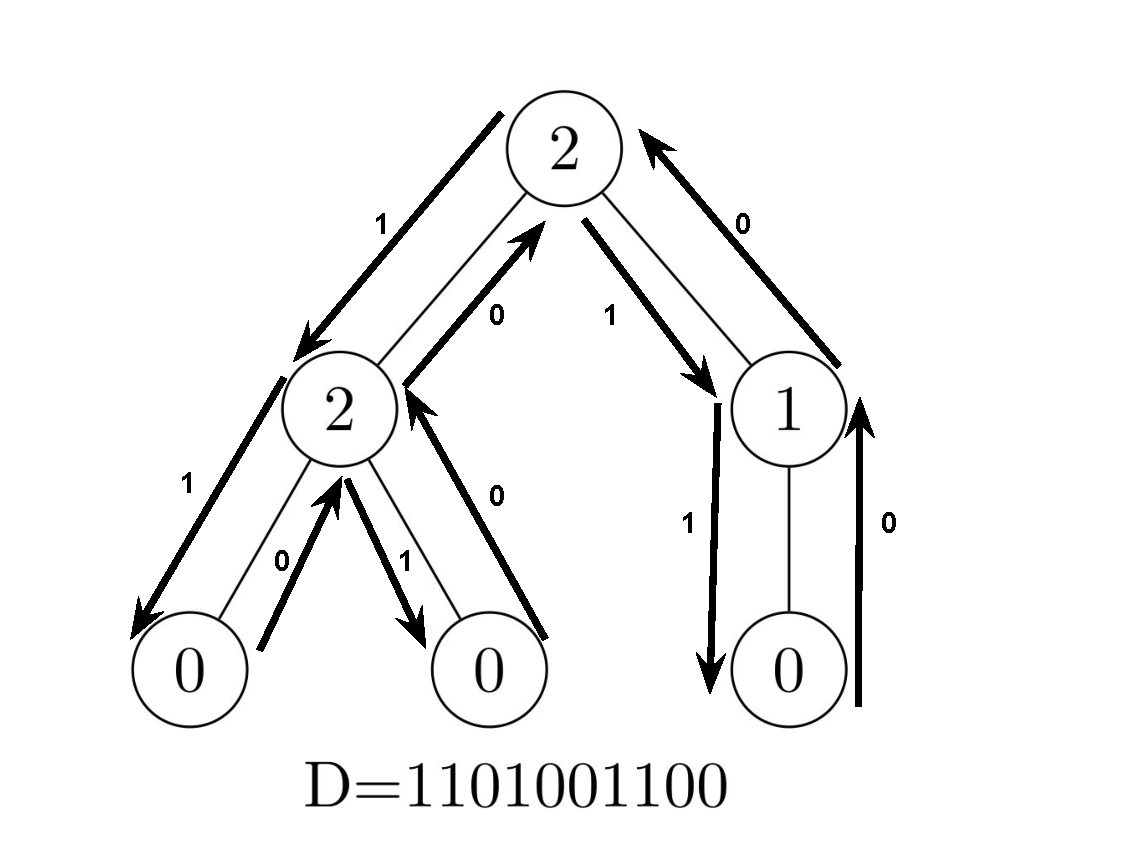
\includegraphics{Ordered-Tree-Bijection-Illustration}
    \caption{An ordered tree with $5+1=6$ nodes corresponding to the order 5 Dyck word $1101001100$.}
    \label{ordered_tree_bijection_illustration}
\end{figure}

%TODO: Combine the above and below figures?? Have them adjacent to each other?

\begin{figure}
    $T=$

    \begin{tikzpicture}[every tree node/.style={draw,circle},sibling distance=10pt, level distance=40pt]
	\tikzset{edge from parent/.style={draw, edge from parent path=
	{(\tikzparentnode) -- (\tikzchildnode)}}}
	\Tree [.\node[style={fill=lightpurple}]{}; [.\node[style={fill=lightpurple}]{G}; [.\node[style={fill=lightpurple}]{P};[.\node[style={fill=lightpurple}]{L}; [.\node[style={fill=lightpurple}]{}; [.\node[style={fill=lightpurple}]{}; [.\node[style={fill=lightpurple}]{F}; ] ] ] ] [.\node{O}; [.\node{}; ] ] [.\node{}; ] ] [.\node{}; [.\node{}; ] ] ] ]
    \end{tikzpicture}

    $D=[1, 1, 1, 1, 1, 1, 0, 0, 0, 0, 1, 1, 0, 0, 1, 0, 0, 1, 1, 0, 0, 0]$
    \caption{An ordered tree with 12 nodes corresponding to the Dyck word 1111110000110010011000.  Each node is labelled with its number of children; the left down path of T is highlighted in purple. Nodes are labelled by their degree.}
    \label{exampleotree}
\end{figure}

In addition to the above bijection, we define the following functions relating to ordered trees, Dyck words, and the correspondence between them.

\begin{itemize}
    \item Let $\otree{D}$ and $\dyck{T}$ be functions that convert a Dyck word to an ordered tree and an ordered tree to a Dyck word respectively via the above process.
    \item Let $\depth{t_i}=$ length of path between root and $t_i$. $\depth{root}=0$
    \item Let $\oneindex{D}{i}=$ be the index of the $i\thh{}$ one in D.
\end{itemize}

\bigskip


The following remarks can be derived from the bijection between ordered trees and Dyck words.


\begin{remark}
    $t_i$ corresponds to the $i$th one in D for $1 \le i \le n$
\end{remark}
\begin{proof}
    Recall the method of constructing an ordered tree from a Dyck word.  Each one in D creates a new node; zeroes in D do not create nodes.  Generating an ordered tree from a Dyck word generates the nodes of the tree in preorder.  Thus, $t_i$ corresponds to the $i$th one in D for $1 \le i \le n$.
\end{proof}

\begin{remark} \label{re:depthformula}
    The relatoinship between...

    % TODO: eqref?
    \begin{equation}
    	\depth{t_i}=\depth{t_{i-1}}+1-(\oneindex{D}{i}-\oneindex{D}{i-1}-1) 
    \end{equation}
    

    Equivalently, $\oneindex{D}{i} = \oneindex{D}{i-1} + \depth{t_{i-1}} - \depth{t_i} + 2$
\end{remark}
\begin{proof}

    Note that $(\oneindex{D}{i}-\oneindex{D}{i-1}-1)$ is equal to the number of zeroes between the $i\thh$ and $(i-1)^{\underline{st}}$ ones in D.  Therfore, this rule can be informally described as follows:

    The depth of $t_i$ is the depth of $t_{i-1}$ plus 1 minus the number of zeroes between the $(i-1)\thh$ and $i\thh$ ones in D

    The number of zeroes between the $i\thh$ and $(i-1)\thh$ ones in $D$ is equal to one plus the depth  $\depth{t_i}$ minus $\depth{t_{i-1}}$

    This follows naturally from the bijection between Dyck words and ordered trees.  Each zero corresponds to a step up in the tree before adding the next child.  

    If there are zero zeroes between the $i\thh$  and $(i-1)^{\underline{st}}$ ones in D, $t_i$ is a child of $t_{i-1}$; $\depth{t_i}=\depth{t_{i-1}}+1$

    If there is one zero between the $i\thh$  and $(i-1)^{\underline{st}}$ ones in D, $t_i$ is a child of $t_{i-1}$'s parent; $\depth{t_i}=\depth{t_{i-1}}+1$.  

    Each subsequent zero between $t_{i-1}$ and $t_i$ decreases $\depth{t_{i}}$ by one.  Thus, the depth of $t_i$ is the depth of $t_{i-1}$ plus 1 minus the number of zeroes between $t_{i-1}$ and $t_{i}$.
\end{proof}
% \bigskip


\begin{remark}A preorder listing of $\depth{t_i} $ for each $ t_i \in T$ can be used to construct a Dyck word. \label{re:construct_dyck}

\end{remark} 
\begin{proof}
    % This follows from Remark \ref{re:depthformula}, as it implies that for any $i,i+1 \le n$, $\oneindex{D}-\oneindex{$ 

    Let $T=t_0,t_1,...t_n$ be a preorder traversal of T.  Note that $t_0$ is the root of $T$

    Construct D as follows: 

    \begin{itemize}
	% \item skip $t_0$
	\item Let $D=\epsilon$ % clear that this is empty string?
	\item For each $t_i$, $1\le i \le n$
	    \begin{itemize}
		\item Append a 1 to $D$
		\item Append $1-\depth{t_{i}}+\depth{t_{i-1}}$ zeroes to D.
	    \end{itemize}
	\item Append $\depth{t_{n}}$ zeroes to D. 
    \end{itemize}
\end{proof} 
\subsection{Successor Rule}

Let $F$ be the leftmost leaf of T, or equivalently the leftmost descendant of the root. Consider the unique path between the root of T and $F$, denoted $\path{T}{root}{F}$. We will refer to this path as the left-down path of T $\leftdown{T}$

% path to leftmost descendent
% Define the left-down path of an ordered tree T, denoted $\leftdown{T}$ to be the first $s+1$ nodes in a preorder traversal of T such that, for each $t_i$ with $0 \le i \le s$, $i=0$ or $t_i$ is the leftmost child of $t_{i-1}$.

Given an ordered tree T, let O be the first node in a preorder traversal of T that is not in the $\path{T}{root}{F}$. Let P be O's parent.  Let G be P's parent, and let L be P's leftmost child (or, equivalently, O's left sibling).  The labels P, G, and L are mnemonics for O's (p)arent, (g)randparent, and (l)eft sibling. 
Fig. \ref{exampleotree} gives an example illustrating O,P,G,L,F, and the left-down path in an tree.

The successor rule for enumerating ordered trees with n nodes can be stated as folows:

\begin{subnumcases}{\nextTree{T} = \label{eq:otreeRule}}
    \treeshift{\treeshift{T}{L}{G}}{O}{root}& if $P \ne root $ and O has no children \label{eq:otree_zeroshift}\\
    \treeshift{T}{L}{O} & otherwise \label{eq:otree_oneshift}
\end{subnumcases}


\begin{subnumcases}{\nextTree{T} = \label{eq:otreeRule_cyclic}}
    \treeshift{T}{F}{root} & $\leftdown{T}=T$ \label{eq:otree_noo_cyclic}\\
    \treeshift{\treeshift{T}{L}{G}}{O}{root}& if $P \ne root $ and O has no children \label{eq:otree_zeroshift_cyclic}\\
    \treeshift{T}{L}{O} & otherwise \label{eq:otree_oneshift_cyclic}
\end{subnumcases}

The following remarks can be derived from from the definition of the successor role and the nodes O,G,L, and T.


Let $D=\dyck{T}$; $s$ be the number of consecutive ones to start D, and $z$ be the number of consecutive zeroes starting at $d_{s+1}$.  Note that $z=(k-s-1)$; $d_{k}=1$

\begin{remark} $\depth{O}=s-z+1$ \label{re:o_depth_formula}
    % \bigskip
\end{remark} 
\begin{proof}


    $t_s$ is the last node in the $\leftdown{T}$, as the left-down path has $s+1$ nodes starting at $t_0$. $t_s$ has depth s, as it is exactly s steps from the root.  Note that $O=t_{s+1}$.  The number of zeroes between $t_s$ and $t_{s+1}$ is the number of zeroes between the $s\thh$ and $(s+1)^{\underline{st}}$ ones in $D_i$.  

\end{proof} 
\begin{remark}O corresponds to $D_k$, i.e. $\oneindex{D}{s+1}=k$
\end{remark}
\begin{proof}
    Let $D=\dyck{T}$ and let k be the index of the 1 in the leftmost 01 substring of D.  Let $t_0...t_s=\leftdown{T}$; $O=t_{s+1}$.

    % TODO: (This can be done better) 

    Note that each 1 in D corresponds to a step down; each 0 to a step up.  Consequently, $\leftdown{T}$ corresponds to the ``all-one" prefix of D.  In other words, $\leftdown{T}=t_0,t_1,...t_{s}$ such that $i=0$ or $D_i=1$. Note that $t_{s+1}$ is therefore the first node in a preorder traversal of T such that $D_{\oneindex{D}{s+1}}=1$ and $D_{\oneindex{D}{s+1}-1}=0$.  O is therefore also the first node in a preorder traversal of T such that $t_{s+1} \notin \leftdown{T}$.  Therfore, $\oneindex{D}{s+1}=k$, i.e., $t_{s+1}=O$ corresponds to the 1 in the leftmost 01 substring of D.

\end{proof}
\begin{remark} Every non-leaf node below P in $\leftdown{T}$ has exactly 1 child.  
\end{remark}

\begin{proof}
    Suppose by way of contradiction that a node below P in $\leftdown{T}$ had a second child. That child would not be in $\leftdown{T}$ and would be be traversed before O in preorder. O was specified to be the first node in a preorder traversal of T that is not in $\leftdown{T}$, which generates a contradiction.

\end{proof}

\begin{remark} \label{re:L_sz1}
    $L$ corresponds to $D_{s-z+1}$, i.e. $\oneindex{D}{s+1}=k$
\end{remark}
\begin{proof}

    $\depth{L}=\depth{O}=s-z-1$ since L and O are siblings. Therefore, L must be $s-z-1$ steps down from the root $\implies$ $L$ is the $s-j-1$th node in a preorder traversal of T $\implies$ T corresponds to $D_{s-z-1}$.


\end{proof}

\subsection{Proof of Correctness} 



% \end{enumerate}

Ruskey and Williams proved that, given a Dyck word of order n, \ref{eq:prefixDyck} iteratively generates all Dyck words of order n.  This proof will use the bijection between Dyck words of order $n$ and ordered trees with $n+1$ nodes to show that that \ref{eq:otreeRule} generates all ordered trees with a given number of nodes.  

Recall that the successor rule $\coolCat{D}$ generates all Dyck words.  Therefore,  To prove that $\nextTree{T}$ generates all ordered trees with $|T|$ nodes, it is sufficient to show that, given an arbitrary ordered tree T, 

\begin{theorem}
    Given an ordered tree T, $\nextTree{T}=\otree{\coolCat{\dyck{T}}}$
\end{theorem}

\begin{proof}




% First, consider the node O in the specification of the $\nextTree{T}$ algorithm.  




$\coolCat{D}$ and $\nextTree{T}$ are each broken down into 3 cases in equations \ref{eq:prefixDyck} and \ref{eq:otreeRule} respectively. 

For convenience, equations \ref{eq:expandedOtree} and \ref{eq:expandedDyck}  give the expanded restatemtents of the successor rules for $\nextTree{T}$ and $\coolCat{D}$ to facilitate comparisons between the two.  %Recall that $s$ is the number of consecutive ones at the start of $D$.

\begin{subnumcases}{\nextTree{T} = \label{eq:expandedOtree}}
    \treeshift{T}{F}{root} & $\leftdown{T}=T$ \label{eq:ex_otree_n}\\
    \treeshift{T}{L}{O} & if O has at least 1 child \label{eq:ex_otree_k1_1} \\
    \treeshift{\treeshift{T}{L}{G}}{O}{root}& if $P \ne root $ and O has no children \label{eq:ex_otree_k1_0} \\
    \treeshift{T}{L}{O} & if O has no children and $P=root$ \label{eq:ex_otree_k}
\end{subnumcases}

\begin{subnumcases}{\coolCat{D} = \label{eq:expandedDyck}}
    \preshift{D}{2n} & \text{if $D$ has no $01$ substring} \label{eq:expandedDyck_n}\\
    \preshift{D}{k+1} & $D_{k+1}=1$ \label{eq:expandedDyck_k1_1}\\
    \preshift{D}{k+1} & $D_{k+1}=0$ and $s>\frac{k-1}{2}$ \label{eq:expandedDyck_k1_0}\\
    \preshift{D}{k} & $D_{k+1}=0$ and $s=\frac{k-1}{2}$ \label{eq:expandedDyck_k}
\end{subnumcases}


% \footnote{important: 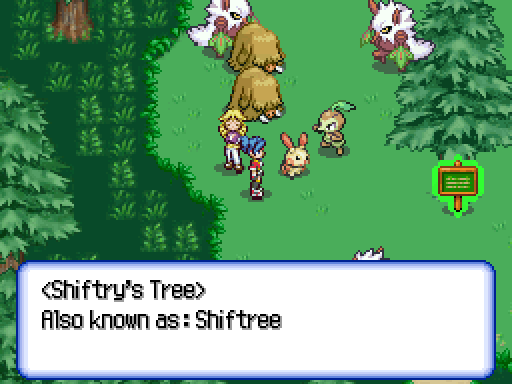
\includegraphics[width=.3\textwidth]{shiftree}} 


We will show the following equivalences:

\begin{itemize}
    \item \ref{eq:ex_otree_n} corresponds to \ref{eq:expandedDyck_n}
    \item \ref{eq:ex_otree_k1_1} corresponds to \ref{eq:expandedDyck_k1_1}
    \item \ref{eq:ex_otree_k1_0} corresponds to \ref{eq:expandedDyck_k1_0}
    \item \ref{eq:ex_otree_k} corresponds to \ref{eq:expandedDyck_k}
\end{itemize}

To accomplish this, we will first prove a few auxillary lemmas to be used to show equivalency between cases. 

Let $D=\dyck{T}$, $s$ be the number of consecutive ones to start D, and $z$ be the number of consecutive zeroes starting at $d_{s+1}$.  Note that $z=(k-s-1)$; $d_{k}=1$
% \begin{itemize}
\begin{lemma} \label{le:final_case_equivalence}

    $D$ has no 01 substring $\iff$ $LD(T)=T$
\end{lemma}
\begin{proof}


    If $D$ has no $01$ substring, $D=1^n0^n$, and T is $n+1$ nodes where $t_0$ is the root and each $t_i$ for $1\le i \le n$ is a child of $t_{i-1}$  In this case, $T$ is a single path of $n+1$ nodes, and the left-down path of T is the entire tree.
\end{proof}
\begin{lemma} \label{le:no_children_equivalence}
    $D_{k+1} = 0 \iff O$ has no children
\end{lemma}
\begin{proof}

    This follows logically from the bijection between Dyck words and ordered trees.  $D_k$ corresponds to O.  If $D_{k+1}=0$, an ``upward" step is taken after O and consequently the next node after O cannot be a child of O.  Since the ones in $D$ give the nodes of T in preorder, O must have no children.

    Informally, once you go ``up" from O, the bijection between Dyck words and ordered trees gives no way to go ``back down" to give O an additional child.
\end{proof}
\begin{lemma} \label{le:tight_case_equivalence}
    $P=root \iff s=z=\frac{k-1}{2}$.
\end{lemma}
\begin{proof}

    First, note that $P=root$ simply means that O is a child of the root.  O is a child of the root $\iff \depth{O}=1$.  Additionally, note that $s+z=k-1$

    As shown in remark \ref{re:o_depth_formula}, $\depth{O}=s-z+1$. Therefore, $P=root \iff s=z=\frac{k-1}{2}$
    i.e. the first $k-1$ symbols of D are $\frac{k-1}{2}$ ones followed by $\frac{k-1}{2}$ zeroes. 

    % This equivalence can can be rewriten as follows: 

    % $s=k-s-1$

    % $2s=k-1$

    % $s=\frac{k-1}{2}$



\end{proof}
% \begin{enumerate}
\begin{lemma}
    \ref{eq:ex_otree_n} corresponds to \ref{eq:expandedDyck_n}
\end{lemma}
\begin{proof}

    Let $D=\dyck{T}$

    Per lemma \ref{le:final_case_equivalence} $D$ has no 01 substring $\iff$ $\leftdown{T}=T$.  

    Thus, $\nextTree{T}$ executes case \ref{eq:ex_otree_n} if and only if $\coolCat{D}$ executes case  \ref{eq:expandedDyck_n}

    Note that since $D$ has no $01$ substring, $D=1^n0^n$. 

    Additionally, since $\leftdown{T}=T$, T can be specified as follows.

    $T=$
    \begin{center}
	\begin{tabular}{ |c|c|c|c|c|c|c|c|c|c|c| } 
	    \hline

	    $node$ & $t_0$ & $t_1$  & $t_2$ & $\dots$ & $t_{n-1}$&$F=t_s=t_n$  \\
	    \hline
	    $depth$ & $0$ & $1$ & $2$ & $\dots$ & $n-1$ & $n$ \\
	    \hline
	    $Dyck$ &  &  \multicolumn{5}{|c|}{$1^n0^n$} \\
	    \hline
	\end{tabular}
    \end{center}

    The third row of this table illustrates the construction of $\dyck{T}$ via the process specified in remark \ref{re:construct_dyck}.

    Shifting $F$ to be the first child of the root changes $\depth{F}$ to 1 and does not affect the depth of any other nodes.  Thus, if $T'=\nextTree{T}$, 


    $T=$
    \begin{center}
	\begin{tabular}{ |c|c|c|c|c|c|c|c|c|c|c| } 
	    \hline

	    $node$ & $t_0$ & $F=t_s=t_n$ & $t_1$  & $t_2$ & $\dots$ & $t_{n-1}$  \\
	    \hline
	    $depth$ & $0$ & $1$ & $1$ & $2$ & $\dots$ & $n-1$ \\
	    \hline
	    $Dyck$ &  &  1 &  \multicolumn{4}{|c|}{$01^{n-1}0^{n-1}$} \\
	    \hline
	\end{tabular}
    \end{center}

    Recall that $\coolCat{D}=\preshift{D}{2n}$ if D has no 01 substring. $D_{2n}=0$, and therefore 

    $\coolCat{D}=101^{n-1}0^{n-1}$
     
     Note that this is exactly the Dyck word constructed from $T'$.  Therefore, if D has no 01 substring or $\leftdown{T}=T$, 

     $\otree{\coolCat{D}}=\nextTree{T}$

\end{proof}
\begin{lemma}
    \ref{eq:ex_otree_k1_0} corresponds to \ref{eq:expandedDyck_k1_0}
\end{lemma}
\begin{proof}
    Let $D=\dyck{T}$

    % \begin{itemize}
    Per lemma \ref{le:tight_case_equivalence} $P=root \iff D$ starts with exactly $\frac{k-1}{2}$ ones.  

    It was also previously shown that $D_{k+1}=0 \iff O$ has no children.  
    Thus, $\nextTree{T}$ executes case \ref{eq:otree_zeroshift} 
    if and only if $\coolCat{D}$ executes case   \ref{eq:expandedDyck_k1_0}

    \bigskip

    We now show that the execution of \ref{eq:otree_zeroshift} is equivalent to the execution of \ref{eq:expandedDyck_k1_0} given case a.
    Given $\dyck{T}=D=1^s0^{z}10d_{k+2}d_{k+3}...d_{2n}$, we aim to show that 

    $\dyck{\nextTree{T}}=\coolCat{\dyck{T}}$
    \bigskip

    Note that $\nextTree{T}=\treeshift{\treeshift{T}{L}{G}}{O}{root}$. 

    Let $T'=\treeshift{T}{L}{G}$; $T''=\treeshift{T'}{O}{root}$

    Note that $\nextTree{T}=T''$

    Since $P \ne root$, we know that G, the parent of P, exists. 
    Thus, we can assume that $G,P,L \in \leftdown{T}$.  T can therefore be specified as follows: 



    % this should be a little lemma
    % $T'$ shifts T so that L becomes the first child of G.  Note that L must have exactly 1 child: otherwise L's second child would be traversed earlier in a preorder traversal than O.  The same logic holds for each subtree of L: Each of L's non-leaf descendents must have exactly one child, as otherwise O would not be the first node in a preorder traversal of T not in $\leftdown{T}$.

    \bigskip
    \bigskip

    $T=$
    \begin{center}
	\begin{tabular}{ |c|c|c|c|c|c|c|c|c|c|c| } 
	    \hline

	    $node$ & $t_0$ & $t_1$ & $\dots$ & $G=t_{s-z-1}$ & $P=t_{s-z}$ & $L=t_{s-z+1}$ & $\dots$ & $F=t_s$ & $O=t_{s+1}$ & $\dots$ \\
	    \hline
	    $depth$ & $0$ & $1$ & $\dots$ & $(s-z-1)$ & $(s-z)$ & $(s-z+1)$ & $\dots$ & $s$  & $(s-z+1)$ & $\dots$\\
	    \hline
	    $Dyck$ &  &  \multicolumn{7}{|c|}{$1^s$} &  $0^{z}1$   & $0\dots$\\
	    \hline
	\end{tabular}
    \end{center}
    % Note that $|\leftdown{T'}|=s+1$; as it is nodes $t_0$ through $F$

    Furthermore, recall that L (and all other non-leaf nodes $\in \leftdown{T}$ must have exactly one child.  Therefore, every node below L in $\leftdown{T}$ has its depth reduced by one; no other nodes have their depth affected by this shift. Therefore, T' can be written as follows:

    \bigskip


    $T'=$
    \begin{center}
	\begin{tabular}{ |c|c|c|c|c|c|c|c|c|c|c| } 
	    \hline

	    $node$ & $t_0$ & $t_1$ & $\dots$ & $G=t_{s-z-1}$ & $L=t_{s-z+1}$ & $\dots$ & $F=t_s$ & $P=t_{s-z}$ & $O=t_{s+1}$ & $\dots$ \\
	    \hline
	    $depth$ & $0$ & $1$ & $\dots$ & $(s-z-1)$ & $(s-z)$ & $\dots$ & $s-1$ & $(s-z)$  & $(s-z+1)$ & $\dots$\\
	    \hline
	    $Dyck$ &  &  \multicolumn{6}{|c|}{$1^{s-1}$} &  $0^{z}1$   & $1$ & $0\dots$\\
	    \hline
	\end{tabular}
    \end{center}

    Since L is now G's first child, P changes from being G's first child to G's second child.  P is therefore removed from the left-down path of $T'$, thereby making P the first node in a preorder traversal of $T'$ that is not in the left-down path of $T'$.  
    Therefore, $|\leftdown{T'}|=s$; $O'=P$. % TODO: check this

    % Note in the case where $z=1$, $L=F=t_s$; i.e. L is the leaf of the left-down path of T.

    Recovering a Dyck word from $T'$, we obtain 

    D'=$1^{s-1}0^z110d_{k+2}d_{k+3},\dots,d_{2n}$


    Next, we use $\treeshift{T'}{O}{root}$ to obtain $T'' = \nextTree{T}$

    $\treeshift{T'}{O}{root}$ shifts O to become the first child of the root. Note that we know that O has no children. Consequently, no nodes other than O have their depth affected by this shift. Thus, 

    \bigskip
    \bigskip


    % TODO: tm+2 dots, here and other tables
    $T''=$
    \begin{center}
	\begin{tabular}{ |c|c|c|c|c|c|c|c|c|c|c|c| } 
	    \hline

	    $node$ & $t_0$ & $O=t_{s+1}$ & $t_1$ & $t_2$ & $\dots$ & $G=t_{s-z-1}$ & $L=t_{s-z+1}$ & $\dots$ & $F=t_s$ & $P=t_{s-z}$ & $\dots$ \\
	    \hline
	    $depth$ & $0$ & $1$ & $1$ & $2$ &$\dots$ & $(s-z-1)$ & $(s-z)$ & $\dots$ & $s-1$ & $(s-z)$   & $\dots$\\
	    \hline
	    $Dyck$ &  & $1$ &  \multicolumn{7}{|c|}{$01^{s-1}$} &  $0^{z}1$   & $\dots$\\
	    \hline
	\end{tabular}
    \end{center}


    % Next, recovering a Dyck word from $$
    \bigskip
    \bigskip

    % TODO: refine



    Therefore, since $T''=\nextTree{T}$, $\dyck{\nextTree{T}}=101^{s-1}0^z1\dots$

    Since $\dyck{T}=D=1^s0^{z}10\dots$
    $\ref{eq:expandedDyck_k1_1}$ gives that

    $\coolCat{\dyck{T}}=101^{s-1}0^z1\dots$

    Therefore, we have shown that $\dyck{\nextTree{T}}=\coolCat{\dyck{T}}=101^{s-1}0^z1\dots$
    % \end{itemize}

\end{proof}
\begin{lemma}
    \ref{eq:ex_otree_k1_1} corresponds to \ref{eq:expandedDyck_k1_1}
\end{lemma}
\begin{proof}

    Per \ref{le:no_children_equivalence}, as $O$ has at least 1 child $\iff D_{k+1}=1$.
    % Note that the conditions for \ref{eq:ex_otree_k1_1} and \ref{eq:expandedDyck_k1_1} are equivalent, as $O$ has at least 1 child $\iff D_{k+1}=1$.

    Thus, $\nextTree{T}$ will execute case \ref{eq:ex_otree_k1_1} if and only if $\coolCat{D}$ executes case \ref{eq:expandedDyck_k1_1}

    Therefore, we aim to show that, given O has at least child and $D_{k+1}=1$,

    $\preshift{\dyck{T}}{k+1}=\dyck{\treeshift{T}{L}{O}}$

    Since $D_{k+1}=1$, we can rewrite D as.
    $D=1^s0^z11$


    \noindent $T=$
    \begin{center}
	\begin{tabular}{ |c|c|c|c|c|c|c|c|c|c|c|c| } 
	    \hline

	    $node$ & $t_0$ & $t_1$ & $\dots$ & $G=t_{s-z-1}$ & $P=t_{s-z}$ & $L=t_{s-z+1}$ & $\dots$ & $F=t_s$ & $O=t_{s+1}$ & $t_{s+2}\dots$ \\
	    \hline
	    $depth$ & $0$ & $1$ & $\dots$ & $(s-z-1)$ & $(s-z)$ & $(s-z+1)$ & $\dots$ & $s$  & $(s-z+1)$ & $s-z+2 \dots$\\
	    \hline
	    $Dyck$ &  &  \multicolumn{7}{|c|}{$1^s$} &  $0^{z}1$   & $1\dots$\\
	    \hline
	\end{tabular}
    \end{center}

    Shift L to be O's first child:

    Nodes $L=t_{s-z+1}$ through $F=t_s$ will now come after O in preorder traversal.  Additionally, $\leftdown{T}$ will now go through O; every node in $\path{T}{L}{F}$ will have its depth increased by one.  

    Therefore, $T'=\nextTree{T}$ can be specified as follows: 

    \noindent $T'=$
    \begin{center}
	\begin{tabular}{ |c|c|c|c|c|c|c|c|c|c|c|c| } 
	    \hline

	    $node$ & $t_0$ & $t_1$ & $\dots$ & $G=t_{s-z-1}$ & $P=t_{s-z}$ & $O=t_{s+1}$ & $L=t_{s-z+1}$ & $\dots$ & $F=t_s$  & $t_{s+2}\dots$ \\
	    \hline
	    $depth$ & $0$ & $1$ & $\dots$ & $(s-z-1)$ & $(s-z)$ & $(s-z+1)$ & $(s-z+2)$ & $\dots$ & $s+1$  & $s-z+2 \dots$\\
	    \hline
	    $Dyck$ &  &  \multicolumn{8}{|c|}{$1^{s+1}$}  & $0^{z}1\dots$\\
	    \hline
	\end{tabular}
    \end{center}

    Note that $z \ge 1$, so $z$ zeroes occur between the one corresponding to $t_{s}$ and the one corresponding to $t_{s+2}$.


    Next, recall that $D=\dyck{T}=D=1^s0^z11\dots$ and that $k=s+z+1$

    Therefore, $\coolCat{D}=\preshift{D}{k+1}=1^{s+1}0^z1\dots$, which is the same as the Dyck word resulting from translating $T'=\nextTree{T}$ to the Dyck word $1^{s+1}0^z1\dots$

\end{proof}
\begin{lemma}
    \ref{eq:ex_otree_k} corresponds to \ref{eq:expandedDyck_k}
\end{lemma}
\begin{proof}

    $T \ne \leftdown{T} \iff D$ has a 01 substring.

    $D_{k+1}=1 \iff O$ has at least one child.

    $D_{k+1}=0$ and $s=\frac{k-1}{2} \iff O$ has no children and O is a child of the root.

    O has no children and P=root. Therefore $s=z$, $k=2s+1$

    We can thus rewrite $D=\dyck{T}=1^s0^s101\dots$

    Furthermore, since $s=z$, O has depth 1. 

    \noindent $T=$
    \begin{center}
	\begin{tabular}{ |c|c|c|c|c|c|c|c|c|c|c|c| } 
	    \hline

	    $node$ & $P=t_0$ & $L=t_1$ & $\dots$ & $F=t_s$ & $O=t_{s+1}$ & $t_{s+2}\dots$ \\
	    \hline
	    $depth$ & $0$ & $1$ & $\dots$ & $s$ & $1$ & $1$ \\
	    \hline
	    $Dyck$ &  &  \multicolumn{3}{|c|}{$1^s$} &  $0^{s}1$   & $01\dots$\\
	    \hline
	\end{tabular}
    \end{center}

    Nodes $L=t_{1}$ through $F=t_s$ will now come after O in preorder traversal.  Additionally, $\leftdown{T}$ will now go through O; every node in $\path{T}{L}{F}$ will have its depth increased by one.  

    Therefore, $T'=\nextTree{T}$ can be specified as follows: 

    \noindent $T'=$
    \begin{center}
	\begin{tabular}{ |c|c|c|c|c|c|c|c|c|c|c|c| } 
	    \hline

	    $node$ & $P=t_0$ & $O=t_{s+1}$& $L=t_1$ & $\dots$ & $F=t_s$  & $t_{s+2}\dots$ \\
	    \hline
	    $depth$ & $0$ & $1$ & $2$ & $\dots$ & $s+1$ & $1$  \\
	    \hline
	    $Dyck$ &  &  \multicolumn{4}{|c|}{$1^{s+1}$} &  $0^{s+1}1\dots$   \\
	    \hline
	\end{tabular}
    \end{center}

Since $D=\dyck{T}=1^s0^s101\dots$, $\coolCat{D}=1^{s+1}0^{s+1}1\dots$ as per case $\ref{eq:ex_otree_k}$.  This is identical to the Dyck word constructed from $T'=\nextTree{T}$.  Therefore, cases \ref{eq:ex_otree_k} and \ref{eq:expandedDyck_k} are equivalent.

\end{proof}

Since these 4 cases cover all cases for the two successor rules, we have shown that $\nextTree{T}=\otree{\coolCat{\dyck{T}}}$ in all cases. 
\end{proof}
\subsection{Loopless Implementation}
todo
